\chapter{Knot Theory}

\section{Torus Knot}

\begin{definition}{Torus Knot}\\
$T_{m,n} : \mathbb{S}^1 \to \mathbb{S}^1 \times \mathbb{S}^1 \subseteq \mathbb{R}^3$ given by $T_{m,n} (z) := (z^m,z^n)$ is called a $(m,n)$-torus knot, i.e.: $m$-times in the longitude and $n$-times in the meridian.
\end{definition}

\begin{proposition}
    $T_{m,n}$ is embedding if and only if $g.c.d.(m,n) =1$.
\end{proposition}

\begin{proof}
    \begin{itemize}
        \item ($\Leftarrow$): Let $\theta ,\theta' \in [0,1)$, s.t.: $\theta \geq \theta'$ $(e^{2\pi i m\theta}, e^{2\pi i n\theta}) = (e^{2\pi i m\theta'}, e^{2\pi i n\theta'})$. Hence, $m(\theta - \theta'), n(\theta - \theta') \in \mathbb{Z}$. Since $\gcd(m,n) =1$, then $\theta - \theta ' \in \mathbb{Z} \Rightarrow \theta = \theta'$. Therefore, $T_{m,n}$ is injective. Obviously $T_{m,n}$ is cont. Then by theorem 4.31, $T_{m,n}$ is embedding.

        \item ($\Rightarrow$): Suppose on the contrary that $d = \gcd (m,n) >1$. Then $m/d,n/d \in \mathbb{Z}$. Hence, $(e^{2 \pi im\theta}, e^{2 \pi in\theta}) = (e^{2 \pi im\theta /d}, e^{2 \pi in\theta/d}) \Rightarrow T_{m,n}$ is not injective, contradiction.
    \end{itemize}
\end{proof}

\begin{theorem}
    $$\Pi_1(T_{m,n}) := \Pi_1(\mathbb{R}^3 \setminus T_{m,n}) \cong \langle a,b \mid a^m =b^n \rangle$$
\end{theorem}

\begin{proof}
    Note that $\mathbb{R}^3 \setminus T_{m,n} \simeq \mathbb{S}^3 \setminus T_{m,n}$.
    \begin{itemize}
        \item \textit{Step 1:}
        \begin{align*}
            \mathbb{S}^3 &= \partial \mathbb{D}^4 \simeq \partial (\mathbb{D}^2 \times \mathbb{D}^2) = \overline{\mathbb{D}^2 \times \mathbb{D}^2} - int(\mathbb{D}^2 \times \mathbb{D}^2) = \overline{\mathbb{D}^2} \times \overline{\mathbb{D}^2} - (\mathbb{D}^2)^\circ \times (\mathbb{D}^2)^\circ\\
            &= (\overline{\mathbb{D}^2} - (\mathbb{D}^2)^\circ) \times \mathbb{D}^2 \cup \mathbb{D}^2 \times (\overline{\mathbb{D}^2} - (\mathbb{D}^2)^\circ) = \partial \mathbb{D}^2 \times \mathbb{D}^2 \cup \mathbb{D}^2 \times \partial \mathbb{D}^2\\
            &= \mathbb{S}^1 \times \mathbb{D}^2 \cup \mathbb{D}^2 \times \mathbb{S}^1
        \end{align*}
        
        \item \textit{Step 2:} Denote $T = \mathbb{S}^1 \times \mathbb{D}^2$, $T' = \mathbb{D}^2 \times \mathbb{S}^1$ and $T'' = T \cap T' = \mathbb{S}^1 \times \mathbb{S}^1$. Note that the $T_{m,n}$ is embedded in $T''$ and that $T''\setminus T_{m,n}$ is homotopic to an annulus. Let $x_0 \in T'' \setminus T_{m,n}$ be a basepoint. Both $T$ and $T'$ are homotopic to $\mathbb{S}^1$. Hence, one has
        \begin{equation*}
            \Pi_1(T) \cong \langle a \rangle  , \Pi_1(T') \cong \langle b \rangle ,\Pi_{1}(T'' \setminus T_{m,n}) \cong \langle c \rangle 
        \end{equation*}
        with $i_{1*} (c) = a^m$ and $i_{2*} (c) =b^n$. 

        \item \textit{Step 3:} Then applying SVK, one can get
        \begin{align*}
            \Pi_1(T_{m,n}) &:=\Pi_1(\mathbb{R}^3 \setminus T_{m,n}) \cong \Pi_1(\mathbb{S}^3 \setminus T_{m,n} ) \cong \Pi_1(T) *_{\Pi_{1}(T''\setminus T_{m,n})} \Pi_1 (T')\\
            &= \langle a ,b \mid i_{1*} (c) = i_{2*}(c) \rangle = \langle a,b \mid a^m = b^n \rangle
        \end{align*}
    \end{itemize}
\end{proof}

\section{Kont}

\begin{definition}{Knot}\\
A knot is an embedding of $\mathbb{S}^1$ in $\mathbb{S}^3$ or $\mathbb{R}^3$.
\end{definition}

\begin{definition}{Equivalent Knots}\\
Two knots $K_1,K_2$ are called \textit{equivalent} if there is a continuous map $F: \mathbb{S}^3 \times [0,1] \to \mathbb{S}^3$, s.t.: 
$$F(x,0) = id_{\mathbb{S}^3},F(x,1) \circ K_1 = K_2, \;and\; F(x,t)\;is \;homomorphism\; \forall t$$
\end{definition}

\noindent \textbf{Remark:} It's easy to show that this definition gives an equivalence relation on space of knots.

\begin{definition}{Tame Knot}\\
Knot $K$ is called tame if its projection in $\mathbb{R}^2$ have finitely many \textit{crossings}.
\end{definition}

\noindent\textbf{Example:}
\begin{itemize}
    \item Unknot (= circle)
    \item Trefoil knot ($T_{2,3}$)
    $$\theta \mapsto \begin{pmatrix}
        2+\cos(3\theta) \cos (2\theta)\\
        2+ \cos(3\theta) \sin(2\theta)\\
        -\sin(3\theta)
    \end{pmatrix}$$
    \begin{figure}[htbp]
    \centering
    \begin{tikzpicture}
        \begin{knot}[]
            consider self intersections=true,
            % draft mode=crossings, % 调试时可取消注释此行，用于查看交叉点的编号
            flip crossing=2,        % 翻转第2个交叉点以形成完美的交错结构
            line width=1.5pt,       % 绳子的粗细
            clip width=5,           % 交叉处“下穿”留出的空白间隙大小
        ]
        % 使用贝塞尔曲线绘制对称的三叶结路径
        \strand (0,2) 
            .. controls +(2.2,0) and +(120:-2.2) .. (210:2) 
            .. controls +(120:2.2) and +(60:2.2) .. (330:2) 
            .. controls +(60:-2.2) and +(-2.2,0) .. (0,2);
        \end{knot}
    \end{tikzpicture}
    
    \label{fig:trefoil}
\end{figure}
\end{itemize}

\begin{definition}{Link}\\
A link is an embedding of a disjoint union of finitely many $\mathbb{S}^1$ to $\mathbb{S}^2$ or $\mathbb{R}^3$.
\end{definition}

\noindent\textbf{Example:} 
\begin{itemize}
    \item Hopf link
    \begin{figure}[htbp]
    \centering
    \begin{tikzpicture}
        \begin{knot}[
            consider self intersections=true,
            % draft mode=crossings, % 如果需要调试上下关系，取消注释此行
            flip crossing=1,        % 翻转第一个交叉点，形成互扣效果
            line width=1.5pt,       % 线条粗细
            clip width=5,           % 上下交错时的留白间隙
        ]
        \strand[darkblue] (0,0) circle (1.2cm);
        \strand[red!80!black] (1.2,0) circle (1.2cm);
        \end{knot}
    \end{tikzpicture}
    
    \label{fig:hopf_link}
    \end{figure}
    \item Bonomean rings
    \begin{figure}[htbp]
    \centering
    \begin{tikzpicture}[scale=1.2]
        \begin{knot}[
            consider self intersections=true,
            % draft mode=crossings,   % 强烈建议在初次编译时取消注释此行，查看交叉点编号
            flip crossing={1, 3, 5},  % 翻转特定编号的交叉点。请根据 draft mode 显示的编号进行调整！
            line width=1.5pt,
            clip width=5,
        ]
        % 使用极坐标定位三个圆的圆心，使它们呈正三角形分布
        \strand[darkblue]      (90:0.7)  circle (1.2cm);
        \strand[red!80!black]  (210:0.7) circle (1.2cm);
        \strand[green!60!black](330:0.7) circle (1.2cm);
        \end{knot}
    \end{tikzpicture}
    
    \label{fig:borromean_rings}

\end{figure}
\end{itemize}

\noindent\textbf{Remark:} When $m,n$ are NOT coprime integers, one has shown that $T_{m,n}$ becomes torus link, with the number of component given by $\gcd(m,n)$.

\section{Wirtinger Presentation of Knot Group}

\begin{figure}[htbp]
    \centering
    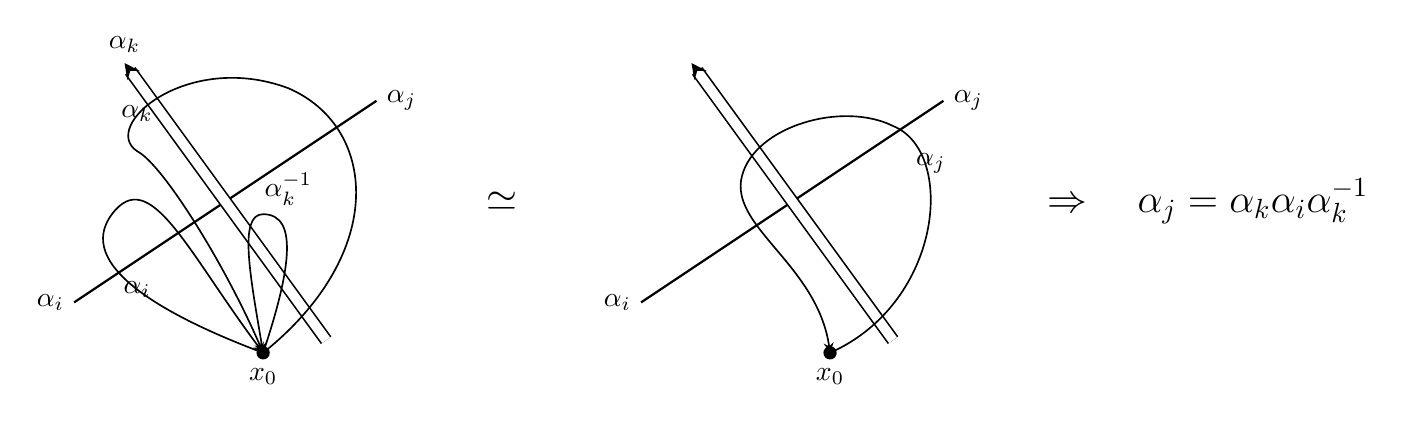
\begin{tikzpicture}[>=stealth, scale=1.6]

        % ==================== 左侧复杂回路图 ====================
        \begin{scope}[shift={(0,0)}]
            % 基准负交叉线 (底层线：左下到右上)
            \draw[thick] (-1.2,-0.8) node[left] {$\alpha_i$} -- (1.2,0.8) node[right] {$\alpha_j$};
            
            % 基准负交叉线 (顶层线：右下到左上，带遮罩)
            \draw[thick, double=white, double distance=3.5pt, line width=0.6pt, ->] (0.8,-1.1) -- (-0.8,1.1) node[above] {$\alpha_k$};
            
            % 基点 x_0
            \coordinate (X0) at (0.3,-1.2);
            \fill (X0) circle (1.5pt) node[below=2pt] {$x_0$};
            
            % Loop \alpha_i (左侧绕线)
            \draw[->, semithick] (X0) .. controls (-0.5,-0.9) and (-1.2,-0.5) .. (-0.9,-0.1) 
                                      .. controls (-0.6,0.3) and (-0.3,-0.4) .. (X0);
            \node at (-0.7,-0.7) {$\alpha_i$};
            
            % Loop \alpha_k^{-1} (右侧小绕线)
            \draw[->, semithick] (X0) .. controls (0.5,-0.6) and (0.6,-0.1) .. (0.3,-0.1)
                                      .. controls (0.1,-0.1) and (0.2,-0.6) .. (X0);
            \node at (0.5,0.1) {$\alpha_k^{-1}$};
            
            % Loop \alpha_k (上方大绕线)
            \draw[->, semithick] (X0) .. controls (1.3,-0.4) and (1.2,0.6) .. (0.5,0.9)
                                      .. controls (-0.3,1.2) and (-1.0,0.6) .. (-0.7,0.4)
                                      .. controls (-0.5,0.3) and (0.0,-0.5) .. (X0);
            \node at (-0.7,0.7) {$\alpha_k$};
        \end{scope}

        % ==================== 中间的同伦等价符号 ====================
        \node at (2.2,0) {\Large $\simeq$};

        % ==================== 右侧变换后的回路图 ====================
        \begin{scope}[shift={(4.5,0)}]
            % 基准负交叉线 (底层线：左下到右上)
            \draw[thick] (-1.2,-0.8) node[left] {$\alpha_i$} -- (1.2,0.8) node[right] {$\alpha_j$};
            
            % 基准负交叉线 (顶层线：右下到左上，带遮罩)
            \draw[thick, double=white, double distance=3.5pt, line width=0.6pt, ->] (0.8,-1.1) -- (-0.8,1.1);
            
            % 基点 x_0
            \coordinate (X1) at (0.3,-1.2);
            \fill (X1) circle (1.5pt) node[below=2pt] {$x_0$};
            
            % Loop \alpha_j (大变形回路)
            \draw[->, semithick] (X1) .. controls (1.2,-0.8) and (1.3,0.4) .. (0.8,0.6)
                                      .. controls (0.4,0.8) and (-0.3,0.6) .. (-0.4,0.2)
                                      .. controls (-0.5,-0.2) and (0.2,-0.5) .. (X1);
            \node at (1.1,0.3) {$\alpha_j$};
        \end{scope}

        % ==================== 最右侧推导公式 ====================
        \node at (7.8,0) {\Large $\Rightarrow \quad \alpha_j = \alpha_k \alpha_i \alpha_k^{-1}$};

    \end{tikzpicture}
\end{figure}

The above figure shows how the formula for negative crossing comes into being. Similarly, we can derive the formula for positive crossing.

\begin{figure}[htbp]
    \centering
    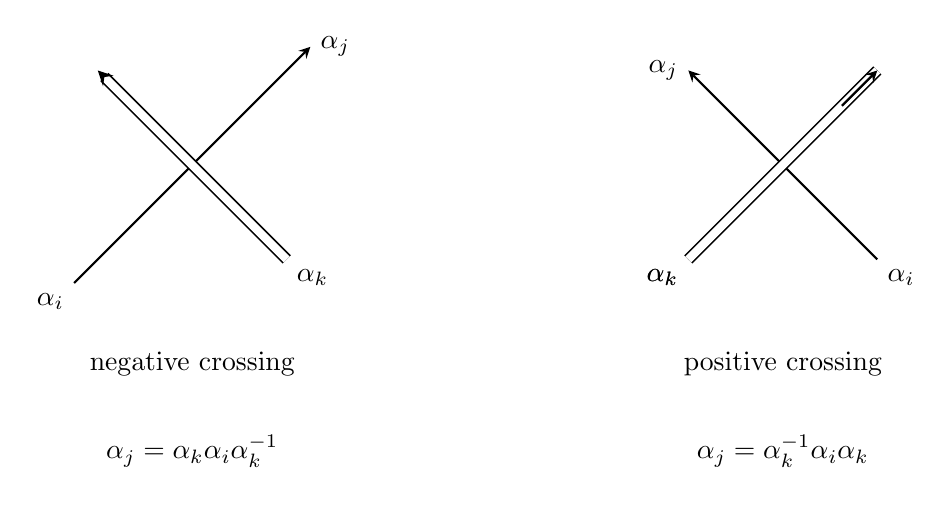
\begin{tikzpicture}[>=stealth, scale=1.5]
        
        % ==================== 左半侧: Negative Crossing ====================
        \begin{scope}[shift={(0,0)}]
            % 被压住的线 (从左下到右上) - 留下空白以模拟被压效果
            \draw[->, thick] (-1,-1) node[below left] {$\alpha_i$} -- (1,1) node[right] {$\alpha_j$};
            
            % 压在上面的线 (从右下到左上) - 使用 double 线条覆盖下面的线
            \draw[->, thick, double=white, double distance=3pt, line width=0.6pt] (0.8,-0.8) node[below right] {$\alpha_k$} -- (-0.8,0.8);
            
            % 文字与公式描述
            \node[below] at (0,-1.5) {negative crossing};
            \node[below] at (0,-2.2) {$\alpha_j = \alpha_k \alpha_i \alpha_k^{-1}$};
        \end{scope}

        % ==================== 右半侧: Positive Crossing ====================
        \begin{scope}[shift={(5,0)}]
            % 压在上面的线 (从左下到右上) - 这次是这条线在上面
            \draw[thick] (-0.8,-0.8) node[below left] {$\alpha_k$} -- (0.8,0.8);
            \draw[->, thick] (0.5,0.5) -- (0.8,0.8);
            
            % 被压住的线 (从右下到左上) - 使用 double 线条，但注意原图是这条被压
            % 为了完美模拟右图（右下到左上的线被压住），我们先画右下到左上，再用 double 画左下到右上
            \draw[->, thick] (0.8,-0.8) node[below right] {$\alpha_i$} -- (-0.8,0.8) node[left] {$\alpha_j$};
            \draw[thick, double=white, double distance=3pt, line width=0.6pt] (-0.8,-0.8) node[below left] {$\alpha_k$} -- (0.8,0.8);
            \draw[->, thick] (0.5,0.5) -- (0.8,0.8); % 补上箭头
            
            % 文字与公式描述
            \node[below] at (0,-1.5) {positive crossing};
            \node[below] at (0,-2.2) {$\alpha_j = \alpha_k^{-1} \alpha_i \alpha_k$};
        \end{scope}
        
    \end{tikzpicture}
\end{figure}

For $l$ arcs in knot diagram with $n$-crossings, the group is given by presentation
$$\langle \alpha_1 ,\cdots, \alpha_l \mid r_1 ,\cdots, r_n \rangle \cong F_l /N_n$$

\noindent\textbf{Example:} Trefoil knot ($T_{2,3}$):

\begin{figure}[htbp]
    \centering
    \begin{tikzpicture}[scale=1.5]
        % 使用 knots 环境绘制三叶结主体，确保完美的上下交错结构
        \begin{knot}[
            consider self intersections=true,
            % draft mode=crossings, % 如果编译后发现上下交错不对，可以取消注释此行查看交叉点编号
            flip crossing=2,        % 翻转第2个交叉点以匹配标准手性
            line width=1.6pt,       % 结的线条粗细
            clip width=5,           % 下穿通过时的空白间隙
        ]
            % 顺时针方向绘制对称的三叶结路径
            \strand (0,2) 
                .. controls +(2.2,0) and +(120:-2.2) .. (210:2) 
                .. controls +(120:2.2) and +(60:2.2) .. (330:2) 
                .. controls +(60:-2.2) and +(-2.2,0) .. (0,2);
        \end{knot}

        % ==================== 1. 顺时针箭头与弧段标签 (\alpha, \beta, \gamma) ====================
        
        % 顶部 \gamma 弧段：在最上方绘制一个顺时针方向的微型箭头
        \draw[thick, ->, >=stealth] (-0.15, 2.0) -- (0.15, 2.0);
        \node[above=3pt] at (0, 2.0) {$\gamma$};

        % 右侧 \beta 弧段：在右下方外侧绘制一个顺时针向下的微型箭头
        \draw[thick, ->, >=stealth] (1.45, -0.6) -- (1.25, -0.9);
        \node[right=4pt] at (1.45, -0.7) {$\beta$};

        % 左侧 \alpha 弧段：在左下方外侧绘制一个顺时针向左下的微型箭头
        \draw[thick, ->, >=stealth] (-1.25, -0.9) -- (-1.45, -0.6);
        \node[left=4pt] at (-1.5, -0.8) {$\alpha$};

        % ==================== 2. 交叉点旁的减号 ($-$ ) ====================
        % 根据三叶结的几何中心，在三个 Crossing 的外侧分别精确标注减号
        
        \node[font=\large\bfseries] at (-0.8, 0.4) {$-$};  % 左侧交叉点旁
        \node[font=\large\bfseries] at (0.8, 0.4) {$-$};   % 右侧交叉点旁
        \node[font=\large\bfseries] at (0, -0.8) {$-$};   % 底部交叉点旁

    \end{tikzpicture}
    
    \label{fig:labeled_trefoil}
\end{figure}

We have 3 negative crossings, so we can get three relations:
$$\alpha = \beta \gamma \beta^{-1},\beta = \gamma \alpha \gamma^{-1}, \gamma = \alpha \beta \alpha^{-1}$$
Therefore, we get
$$\Pi_{1} (T_{2,3}) = \langle \alpha,\beta,\gamma \mid \alpha = \beta \gamma \beta^{-1},\beta = \gamma \alpha \gamma^{-1}, \gamma = \alpha \beta \alpha^{-1} \rangle = \langle \alpha,\beta,\gamma \mid \beta = \gamma \alpha \gamma^{-1}, \gamma = \alpha \beta \alpha^{-1} \rangle$$
It's easy to show that the Wirtinger's presentation of $T_{2,3}$ is same as the form in theorem 10.3, i.e.:
$$\langle \alpha,\beta,\gamma \mid \beta = \gamma \alpha \gamma^{-1}, \gamma = \alpha \beta \alpha^{-1} \rangle \cong \langle a,b \mid a^2 = b^3\rangle$$

\section{Seifert-van Kampen Theorem applied to knot group}

For a knot $K$, we firstly fatten $K$ into a tubular neighborhood $nbhd(K)$. Note that $\mathbb{R}^3 \setminus K$ can be deformation retract onto $\mathbb{R}^3 \setminus nbhd(K)$. Since $K$ is compact, then we can take $\mathbb{R}^3 \setminus nbhd(K) = U_1 \cup U_2$ where $U_1 = \{ (x,y,z) \mid z < \epsilon_1 \} \setminus nbhd(K)$ and $U_{2} = \{ (x,y,z) \mid z > \epsilon_2 \} \setminus nbhd(K)$ for some $\epsilon_1,\epsilon_2 \in \mathbb{R}$. Choose basepoint in $U_1 \cap U_2$. Then applying SVK,
$$\Pi_1(\mathbb{R}^3 \setminus K) \cong \Pi_1(U_1) *_{\Pi_1(U_1 \cap U_2)} \Pi_1(U_2)$$
The remaining steps require a case-by-case analysis.